\chapter{Physical Design}
The trend nowadays is to build more complex system (in terms of transistors) in less time (reduce the time-to-market), so there is the need of some powerful tools that allows having optimized ICs. The design flow strategy is based on multi-abstraction 3-step iteration:
\begin{enumerate}
	\item The hardware is described using a Hardware Description Language, as VHDL
	\item The Synthesis phase takes as input the abstract model and generates a more detailed model that contains additional information about timing, power consumption and area. The next step is the Optimization one, which is used in order to generate an equivalent behaviour circuit and at the same time satisfy some conditions, like timing
	\item A post synthesis simulation is run to check the functional properties of the final model
\end{enumerate}
\section{Synthesis}
\label{sec:syn_opt}
The synthesis has been done with intensive script usage; in fact, two scripts have been developed in order to set up the environment, perform the synthesis and clean up all the useless temporary files generated during the process.\newline\newline
The first script is a bash script (refer to Appendix \ref{bash_syn}) and, as anticipated before, it is used to set up the environment by coping the \texttt{.synopsys\_dc.setup} file, copy the library and call the synthesis script suing \texttt{dc\_shell}.
Once the synthesis is over, the bash script removes all temporary folders like \texttt{ARCH}, \texttt{DOBY}, etc \dots and moves the synthesized DLX, in both Verilog and VHDL, and all the generated reports into a specific folder.\newline\newline

The second script, that is run under the \texttt{dc\_shell} to perform the actual synthesis, executes multiple steps (refer to Appendix \ref{tcl_syn}):
\begin{itemize}
	\itemsep0sp
	\item Analyze all the .vhd files needed for the DLX
	\item Elaborate the DLX design, by correctly configuring the generics
	\item Set the wire model and create a clock, that is the constraint
	\item Perform the compilation
	\item Save the synthesized DLX
	\item Save the timing, area and power report 
\end{itemize}
The clock timing, which is set to 2.5 ns, has been selected after many trials and errors, in order to find the lowest possible value. Critical paths, like the one that passes through adder, has been reduced using an optimized design, e.g. P4 adder.\newline\newline
All complete reports are detailed in the Appendix \ref{ap3}; from the area report, it's possible to observe that the total cell area is 35278.25. It is divided into 19747.84 for the combinational part and 15530.41 for the non-combinational one.\newline\newline
Given a timing constraint, another important piece of information that can be extracted from the timing report is the \textit{slack}. It represents the time margin that the worst path has; in this way, the clock in the synthesis script can be reduced as much as possible in order to increase performance.

\section{Place and Route}
The Placement step consists of placing all the block and I/O pins within a defined area that is the chip. After this macro-step all the units are placed and so the routing is performed in order to connect all blocks together. After the place and route are both completed, a simulation ensures that everything is correct. The final result can be observed in Figure \ref{fig:phy_end}.


\begin{figure}[h!]
	\begin{subfigure}[t]{.45\textwidth}
		\centering
		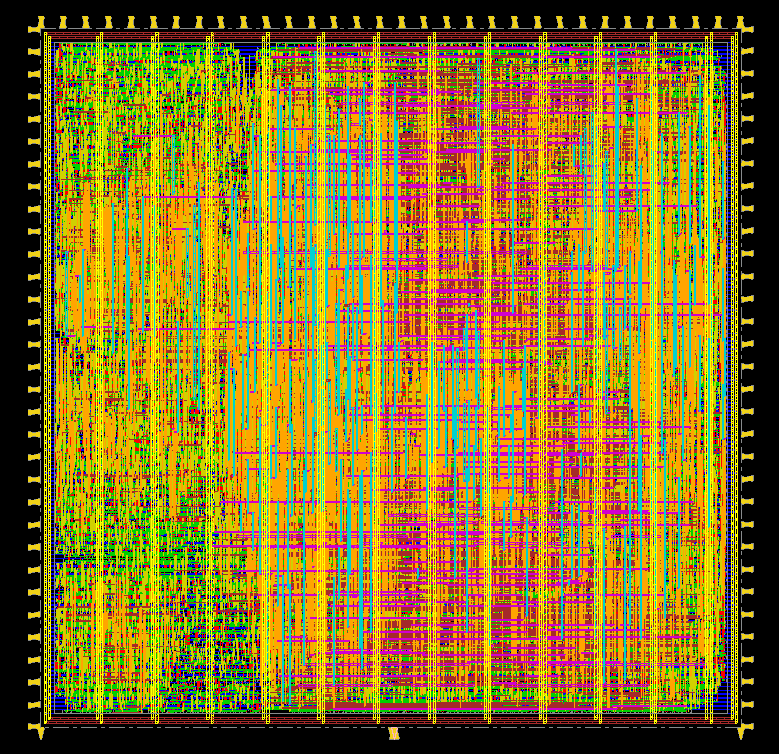
\includegraphics[width=.9\textwidth]{chapters/9_PhysicalDesign/images/pre_routing.png}
		\caption{DLX processor before routing, only logical connections are present}
		\label{fig:pre_routing}
	\end{subfigure}\hfill
	\begin{subfigure}[t]{.45\textwidth}
		\centering
		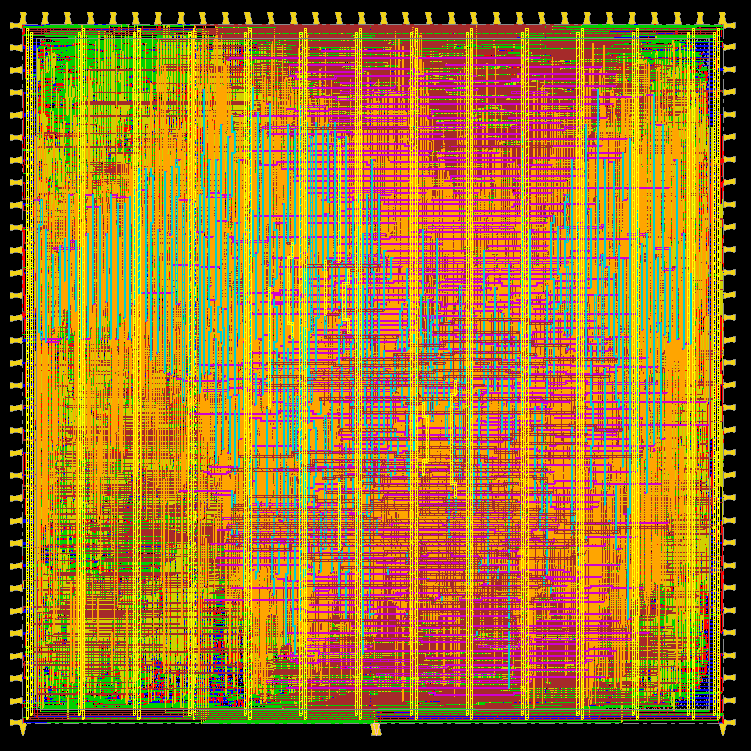
\includegraphics[width=.9\textwidth]{chapters/9_PhysicalDesign/images/phy_end.png}
		\caption{DLX processor after Place and Route phases}
		\label{fig:phy_end}
	\end{subfigure}
	\caption{DLX Place and Route}
\end{figure}

In order to obtain a fully placed and routed DLX, many steps are performed:
\begin{itemize}
	\item Structuring the Floorplan: in this step the Verilog file has been loaded using a global file called \texttt{DLX.globals} and a specif amount of internal area is dedicated to the core, while the external one is used for the power rings;
	\item Power distribution: around the core, two metal rings has been located for distributing the power supply, so both GND and $V_{dd}$. This is not enough, since the power and ground signals must be correctly distributed. For this reason, multiple vertical metal wires, called strips, has been added to the physical layout. There is a trade-off in the number of stripes, since a high number of them could lead to some problems during the cells routing. Moreover, horizontal wires has been placed to prepare $V_{dd}$ and GND for the standard cells. The results are visible in Figure \ref{stripes};
	\begin{figure}[h]   
		\centering
		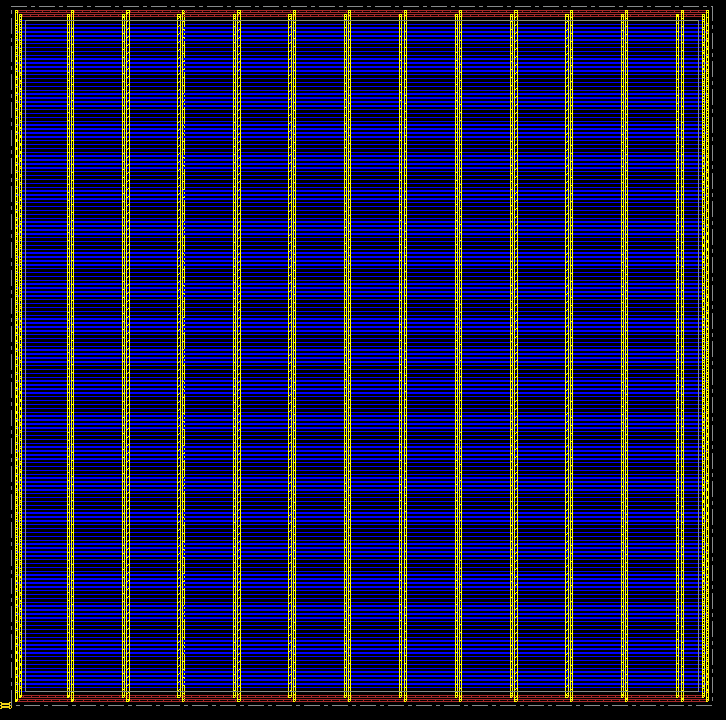
\includegraphics[width=0.38\textwidth]{chapters/9_PhysicalDesign/images/pwr_distribution.png}
		\caption{Result after placing GND and $V_{dd}$ rings with vertical and horizontal stripes.}
		\label{stripes}
	\end{figure}
	
	\item I/O placing: at this point, cells and I/O pins can be placed. Before filling the empty spaces with filler cells a Post Clock-Tree-Synthesis (CTS) optimization has been performed. The result is visible in Figure \ref{fig:pre_routing};
	\item Routing: the last step is the routing; logical interconnections has been replaced with physical interconnections between cells, considering the available stripes and metal rings. The design is now complete, but a post routing optimization has been performed in order to respect the required timing constraints.
\end{itemize}

Once the Place and Route step has been done, a timing analysis has been performed using the \textit{Innovus Debug timing} in order to visualize the delay distribution. The paths delay distributions is visible at \ref{fig:innovus_delay}.
\begin{figure}[h]   
	\centering
	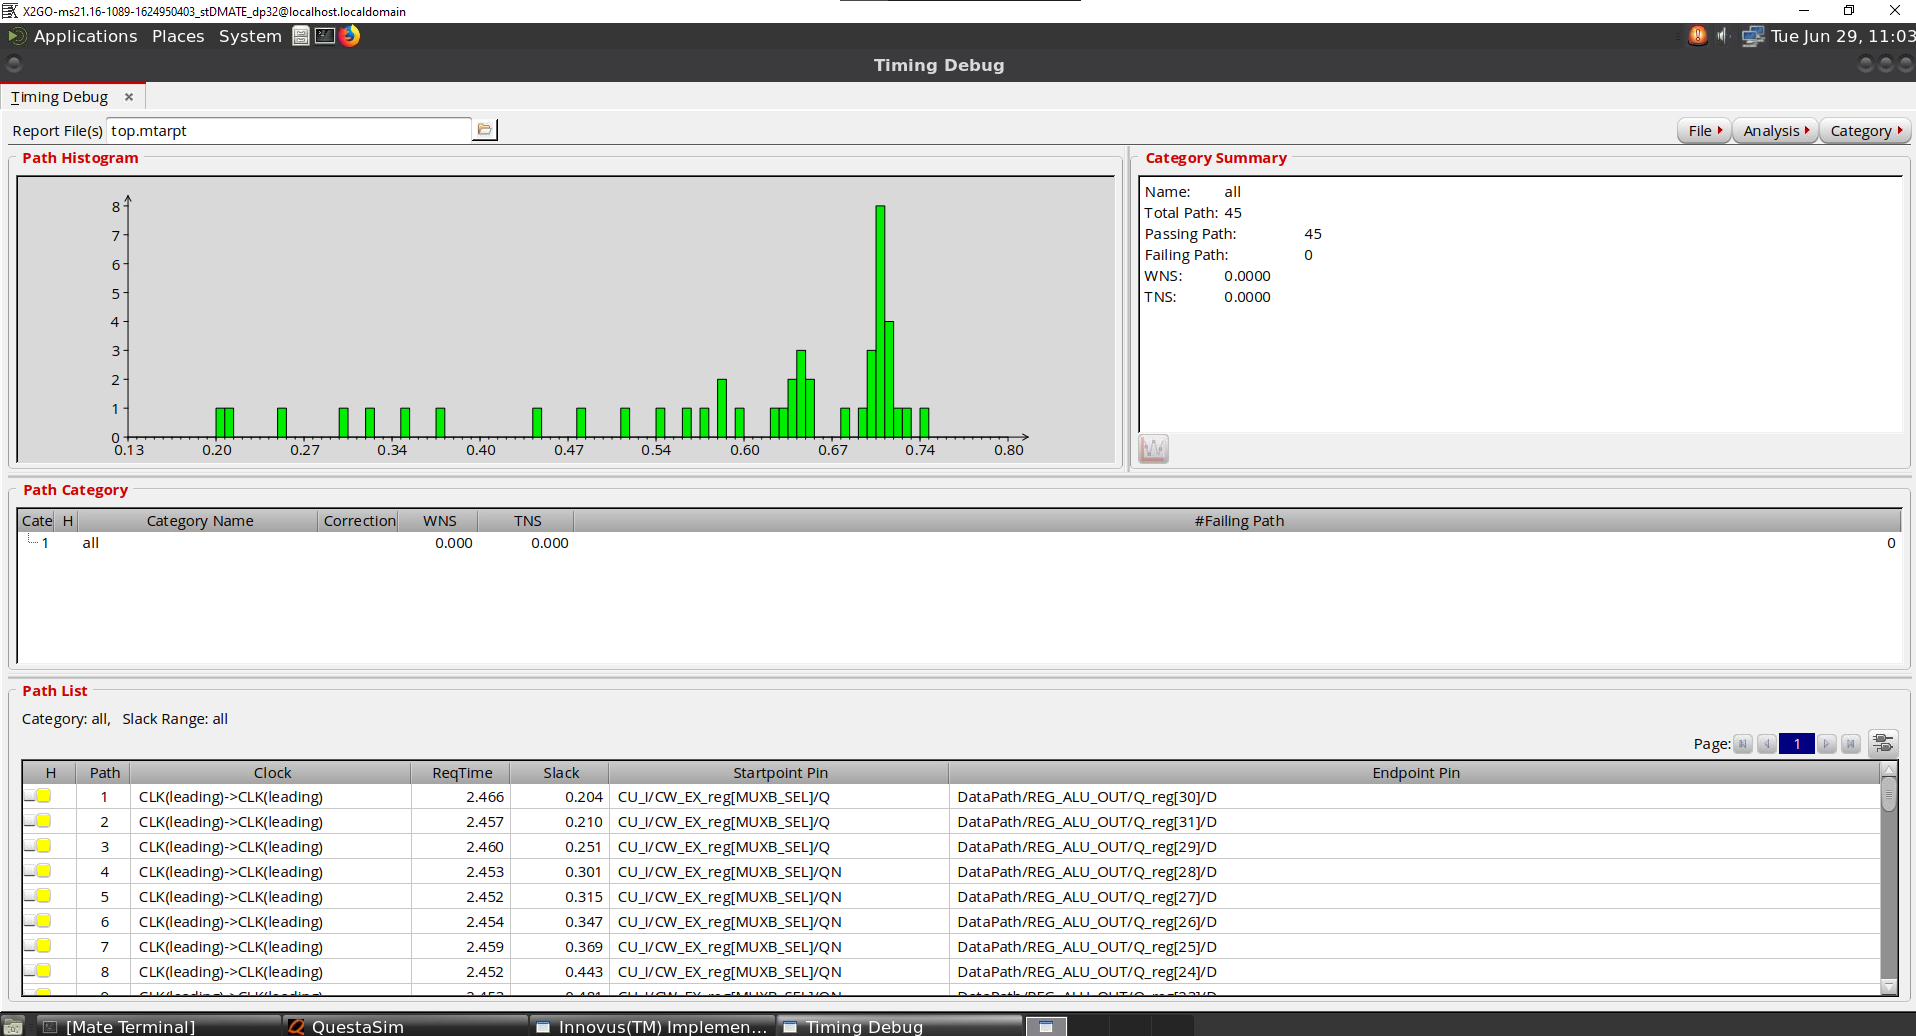
\includegraphics[width=0.8\textwidth]{chapters/9_PhysicalDesign/images/innvous_delay.png}
	\caption{Result after placing GND and $V_{dd}$ rings with vertical and horizontal stripes.}
	\label{fig:innovus_delay}
\end{figure}

Last but not least, before ending the place and route process, a design analysis and verification has been performed in order to ensure that the connectivity and the design rules are respected.